% Author: Animesh Garg
% Date: June 20, 2013
%This document has slightly modified the template from ICRA 2013 website. 

\documentclass[letterpaper, 10 pt, conference]{ieeeconf}  % Comment this line out if you need a4paper
%\documentclass[a4paper, 10pt, conference]{ieeeconf}      % Use this line for a4 paper

\IEEEoverridecommandlockouts                              % This command is only needed if 
                                                          % you want to use the \thanks command
\overrideIEEEmargins                                      % Needed to meet printer requirements.

\usepackage{graphics} % for pdf, bitmapped graphics files
\usepackage{epsfig} % for postscript graphics files
%\usepackage{mathptmx} % assumes new font selection scheme installed
\usepackage{times} % assumes new font selection scheme installed
\usepackage{amsmath} % assumes amsmath package installed
\usepackage{amssymb}  % assumes amsmath package installed

%USER DEFINED PACKAGES
\usepackage{mathtools}
\usepackage{amsfonts}
\usepackage{algorithmic}
\usepackage{setspace}
\usepackage{fancyhdr}
\usepackage{lastpage}
\usepackage{extramarks}
\usepackage{chngpage}
\usepackage{soul}
\usepackage[usenames,dvipsnames]{color}
\usepackage{graphicx,float,wrapfig}
\usepackage{ifthen}
\usepackage{listings}
\usepackage{courier}
\usepackage{graphicx}
\usepackage{epstopdf}

%Do not use both cite and natbib together
%\usepackage{cite}

% the next three lines allow natbib to be used with ieeeconf document style
\makeatletter
\let\NAT@parse\undefined
\makeatother

% numbers option provides compact numerical references in the text. 
\usepackage[sort&compress,numbers]{natbib}

\usepackage{multicol}
\usepackage[bookmarks=true]{hyperref}

%USER DEFINED MACROS
% TODO
\newcommand{\todo}[1]{{ \color{red} {[ToDo:#1]}}}

%Author Comments
\newcommand{\ken}[1]{{ \color{blue} {[Ken: #1]}}}
\newcommand{\AG}[1]{{ \color{cyan} {[AG: #1]}}}
\newcommand{\SP}[1]{{ \color{magenta} {[SP: #1]}}}

%%%%%%%%%%%%%%%%%%%%%%%%%%%%%%%%%%%%%%%%%%%%
%TITLE
\title{\LARGE \bf
Designing Minimum Discomfort Stereotactic Medical Fixtures \\
using Submodular Robot Grasp Coverage Algorithms 
%Exploiting Submodular Grasping for Custom Designed Patient Positioning Systems 
%to improve Radiation Therapy
}

%%%%%%%%%%%%%%%%%%%%%%%%%%%%%%%%%%%%%%%%%%%%%
%AUTHOR LIST
\author{Animesh Garg$^{1}$, Zach Mulder$^{1}$, Nikitha Singh$^{1}$, Sachin Patil$^{2}$, John Schulman$^{2}$, Pieter Abbeel$^{2}$, Ken Goldberg$^{1,2}$% <-this % stops a space
\thanks{*This work is supported by a grant}% <-this % stops a space
\thanks{$^{1}$Department of IEOR, UC Berkeley,
	Berkeley, CA 94720, USA}%
\thanks{$^{2}$Department of EECS, UC Berkeley,
        Berkeley, CA 94720, USA}%
\thanks{{\tt\small \{animesh.garg, sachinpatil, goldberg\} @berkeley.edu}}%
}


\begin{document}

%Keep these as it is, they are from the ICRA template.
\maketitle
\thispagestyle{empty}
\pagestyle{empty}


%%%%%%%%%%%%%%%%%%%%%%%%%%%%%%%%%%%%%%%%%%%%%%%%%%
\begin{abstract}
to be finalized!
\end{abstract}

\noindent \textit{ Keywords -- submodular grapsing, patient positioning, 
external beam radiation therapy}
%%%%%%%%%%%%%%%%%%%%%%%%%%%%%%%%%%%%%%%%%%%%%%%%%%
% Author: Animesh Garg
% Date: June 23, 2013

\section{INTRODUCTION}
\label{sec:introduction}
% Motivate the problem

Every year, \todo{X} cases of cancer are treated with Radiation therapy 
in United States.
External Radiation Therapy, along with its variations, is a common form
of radiotherapy treatment. With external radiation therapy, radiation is usually 
administered as a complex combination radiation beams directed at the tumor. 
Advanced techniques of dose 
calculation and treatment delivery are employed to permit design of treatment 
fields to maximize the differential in dose delivered to tumors and healthy 
tissue.

Accuracy and precision in patient positioning is essential for success of 
external radiation delivery systems. Since radiation therapy is delivered over 
multiple sessions, repeatability of a patient positioning system is important 
to maintain registration between the patient and radiation delivery equipment.

Presently, a variety of patient positioning  systems are employed in clinical 
procedures. However, most if not all of these systems are one-size-fits-all. 
This leads to problems in maintaining conformance between
simulated and physically delivered radiation dose distributions over multiple 
sessions. Furthermore, these patient positioning systems are inconvenient 
for the patients often requiring local anesthesia to relieve pain.

%Give example of the problem
For instance, stereotactic radiotherapy (SRT) is used primarily for treating 
tumors in the brain. The procedure has sub-millimeter accuracy, but assumes 
exact patient to machine registration. Commercially available head positioning 
solutions for SRT usually require the patient's head to be placed in a cubical 
frame with multiple pegs securing the head in its place. One example of such
a system is illustrated in figure~\ref{fig:leskellFrame}. These pegs are 
uncomfortable and the the frame only allows the head to be placed in a 
small set of orientations.

Additionally, the ability to easily position the head in any orientation simplifies
planning for radiation dose in external radiation therapy. For e.g., if a patient 
is immobilized in a non-supine position, reaching tumor might become easier 
due to decreased hindrance from healthy tissue. 


%state our solution
The key insight in building a principled solution for immobilization is 
customization to patient anatomy. We propose a solution which leverages 
redundant point contacts  and uses surface contacts. 
This higher degree of customization is also facilitated by
recent advances in additive manufacturing and 3D printing.

After a 3D reconstruction of the patient anatomy using a CT (or MRI) scan,
we use redundant contact points and surface contacts to the set of minimal 
grasp points required for immobilization. This reduces maximum force at any
contact point. The benefit of inclusion of additional contact points is a 
submodular function, which allows us to find the optimal set in reasonable time. 

%list claims and their significance. (Use forward referencing instead of explicit roadmap of the paper. )
This study builds upon the previous work from Schulman et al 
\cite{schulman2011grasping}. In this paper,
\begin{itemize}
\item We describe an algorithm which minimizes maximum contact force and 
immobilizes the subject.
\item We evaluate the performance of algorithm on multiple instances of \todo{X} 
body parts.
\item We create a patient specific head positioning system using 3D printing.

\end{itemize}

\begin{figure}[t!]
  \begin{center}
    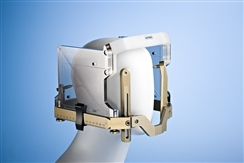
\includegraphics[width=0.8\linewidth]{images/leskellFrame}
  \end{center}
  \vspace{-10pt}
\caption{ The figure shows a Leskell Coordinate Frame G used for Stereotactic Radiosurgery.
As illustrated in the picture, the patient head is placed in a frame and secured in place with 
use of multiple pins}
  \vspace*{-15pt}
  \label{fig:leskellFrame}
\end{figure}

% Author: Animesh Garg
% Date: June 26, 2013

\section{RELATED WORK}
\label{sec:relatedWork}

Grasping and manipulation of real world objects has been studied for over 
a century. The problem of fixturing objects, whether by use of mechanical 
jigs and fixtures, or by actuated robots, has garnered research interest across
disciplines.

A review of Grasping and closure for robotics is provided by 
Bicchi and Kumar \cite{bicchi2000robotic}. A detailed explanatory material 
on grasping has been provided in \cite{prattichizzo2008grasping}. 

As covered in both \cite{2000robotic, prattichizzo2008grasping}, a 
fundamental requirement of grasping and manipulation is to constraint an object 
in equilibrium and control position and orientation of the object as needed. 
Grasp closure has been characterized in two useful manners: Form Closure and
Force Closure. 

The joint vector of forces and moments at a contact point in $\mathbb{R}^3$ is 
called as wrench. An rigid object grasped by a set of rigid contact points 
(may be fixed or actuated), is said to be form closed if it is impossible to 
move the object. Similarly, a rigid object is said to be force closed if an 
arbitrary wrench can be counteracted by a change in contact wrench intensity.
Force closure is similar to form closure but relaxed to allow for friction 
forces to balance object wrenches. 

In applications of fixturing and grasping in healthcare, often form closure
is preferred  over force closure due to use of passive positioning systems. 
For instance in SRT, patient's head is immobilized using a passive device
ensuring no disturbance while treatment is being delivered. 

Markenscoff et al \cite{markenscoff1990geometry} showed that 3D objects with 
piece-wise smooth boundary (including polyhedra) can be form closed in atmost
seven frictionless contacts. We note that choosing this minimal 
set of contact points can result in a high normal contact force at a subset of 
contacts. In medical fixturing, such characteristics of a fixture are 
undesirable because they may lead to localized pain, skin rupture 
and even injury. Hence we propose the use of redundant contacts for form closure. 

\begin{figure}[t!]
  \begin{center}
    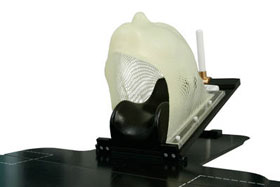
\includegraphics[width=0.75\linewidth]{images/headstep}
  \end{center}
  \vspace{-10pt}
\caption{ The figure shows a Elekta HeadStep used for Stereotactic Radiosurgery.
As illustrated in the picture, the patient head is placed in a frame and secured in place with elstic mask}
  \vspace*{-15pt}
  \label{fig:HeadStep}
\end{figure}

%Related work on grasping with redundant contacts
Modular grasping fixtures have been described by Brost and Goldberg al 
\cite{brost1996complete}. Grasping deformable objects has been a challenge 
in manipulation research. Gopalakrishnan and Goldberg 
\cite{gopalakrishnan2004Dspace} describe new techniques using D-Space for
holding deformable parts. Borst et al \cite{borst1999fast} proposed a 
fast and robust grasp planner. Fast grasp planning and fixturing has since been 
explored by a number of research efforts \todo{find papers}.


Teichmann and Mishra \cite{teichmann2000probabilistic} provided an algorithm for 
grasp quality optimization by a reduction of grasping problem given a set 
of contact points to a convex set cover problem. Ferrari and Canny
\cite{ferrari1992planning} published a seminal work on
geometric grasp quality metrics. They quantified the concepts of total 
force and maximum force as convex hull and minkowsky sum of contact wrenches,
respectively.

Wang \cite{wang2000optimum} proposed an optimal 3D part fixture design 
methodology given a point set of contact points. 

%Related work on medical fixtures
Bale et al \cite{bale1999new} propose a new vaccum based device for
extremity immobilization.
\todo{published works in medical/body part fixturing}

%List commeercial stuff from Elekta
There are a number of commercial medical patient positioning systems currently
used in clinic. As shown in figure~\ref{fig:leskellFrame}, the Leskell coordinate frame G four tapping screws
keep the frame attached to the patient's head. This frame requires local 
anesthesia to minimize patient discomfort during the procedure. 



Figure~\ref{fig:HeadStep} shows a Elekta HeadStep which is used for
immobilization in cranial as well as head, neck and shoulder procedures.
It uses an elastic mask to cover the face and the head with incisions for 
breathing. 


\begin{figure}[t!]
  \begin{center}
    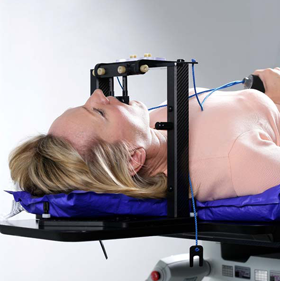
\includegraphics[width=0.9\linewidth]{images/headfix}
  \end{center}
  \vspace{-10pt}
\caption{ The figure shows a Elekta HeadFix used for Stereotactic Radiosurgery.
As illustrated in the picture, the patient head is placed in a frame and secured in place with vacuum activated mouthpiece holding the patients upper jaw.}
  \vspace*{-15pt}
  \label{fig:HeadFix}
\end{figure}


Figure~\ref{fig:HeadFix} shows a Elekta HeadFix which is used for
head immobilization. It uses a vacuum activated head frame system which uses a 
mouthpiece to clamp down the patients upper jaw. The impression of the upper jaw 
is patient specific. 

\todo{
Look up if there are other companies doing similar stuff
Keywords patient positioning in SBRT
}

Our work extends the findings of Schulman et al\cite{schulman2011grasping}
to applications in medical fixturing. Furthermore we also propose a method of 
initial generation of feasible contact points using geometric intuitions from 
local curvature and also no-go zones as specified by a phycisian (viz. mouth, eyes,
ears, nose etc.) Similar methods can also be used for generating form/force
closure grasps for physical objects using multi-fingered hands or multiple hands. 

%Elekta Leskell coordinate frame G requires anaesthetics to minmize patient discomfort.
%Fixing the frame to the patient’s head is simplicity itself - four self-tapping 
%screws keep the lightweight frame firmly and accurately in place, while local 
%anesthesia minimizes any patient discomfort during the procedure.

%Elekta HeadSTEP
%Its excellent robustness and quality guarantees precise and simple 
%repositioning in routine cranial as well as head, neck and shoulder 
%immobilization.
% Author: Animesh Garg
% Date: July 15, 2013

\section{PROBLEM STATEMENT}
\label{sec:problemStatement}

The problem of minimizing discomfort in medical fixtures can be modeled as a 
form closure grasping problem with bounded contact wrench at any contact point.

We are given input a surface mesh,$M$ of the body volume,$V$ required to be 
fixed. The mesh $M$ can be generated using MRI/CT scanning. Gravity vector ($g$) is also provided as input. The required output
 of the algorithm is the subset of points, $S_opt$ on the surface mesh which 
 are required for form closure with bounded contact wrench, $w_ub$. 

Thereafter, only using points in $S_opt$ we construct a fixture, $F$ to hold the 
body volume $V$. The fixture,$F$ is then physically created using 3D-printing. 
The fixture $F$ may consist of multiple pieces, which need assembly over body 
volume $V$. The fixture assembly on the body volume $V$ is in principle 
guaranteed to hold $V$ in form closure. 

\begin{figure}[t!]
  \begin{center}
    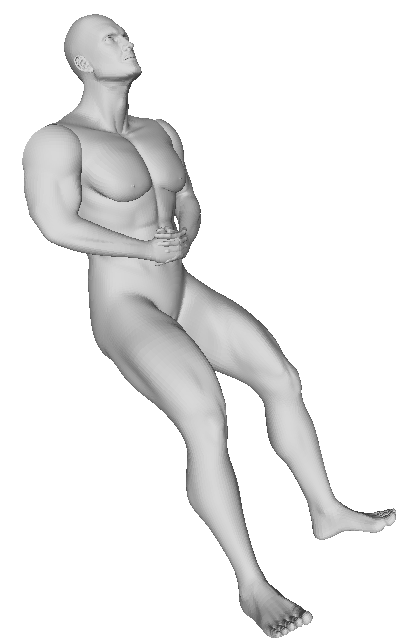
\includegraphics[width=0.6\linewidth]{images/maleBody}
  \end{center}
  \vspace{-10pt}
\caption{ The figure shows a commercially available high fidelity mesh of a human male body. We will use this model for evaluation of proposed algorithmic fixturing techniques in this paper.}
  \vspace*{-15pt}
  \label{fig:maleBody}
\end{figure}


We will evaluate the results using a standard commercially available human body 
mesh for experimentation as shown in figure~\ref{fig:maleBody}\todo{ask Sachin about origins of the model.} Quality 
of algorithmically generated fixtures will be measured for head and limb 
fixturing in virtual environments for varying number of contacts and varying the upper bound on contact wrench, $w_ub$.

Furthermore, we will 3D print the head and a portion of torso to mimic the patient in supine position. We will also create a custom head fixture for physical assessment of the proposed fixtures. 
% Author: Animesh Garg
% Date: June 23, 2013

\section{OUR APPROACH}
\label{sec:Algorithm}


\subsection{Generate Candidate Contact points}
\label{subSec:genContacts}
As observed in the results section, naive uniform sampling of the mesh surface 
for contact point candidates results in pathological contact points. Hence we 
propose the following heuristic approach for generation of contact point 
candidates:
\begin{enumerate}
\item Calculate density of vertices (or faces) around each vertex. 
Alternatively, we can use the valency of each vertex (the number of faces it is 
part of) for estimating the change in curvature in the neighborhood of a 
vertex. 
High density of faces implies complex surface. In case of a human head these 
 would be facial areas like the lips, eyelids, nostrils and ears.

\item Eliminate all candidate vertices (or faces in a mesh), where the normal 
is facing in the mesh or intersects with the mesh in close vicinity. Example 
the back of the ear results in normals pointing in the head. 

\item Weight all vertices, after elimination, inversely proportional to their 
neighborhood density. And now sample from this set. 

\end{enumerate}

We note that facial features in humans are comparatively on the higher side of 
complexity. However the above heuristic would also work for less complex areas 
like elbow and knee. 
Also it is worth noting that noise wrenches would still be sampled uniformly from the mesh. This implies that the gravity can be in any direction or the person can try to move in any direction.

\todo{formalize the contact point sampling}



\subsection{Choice of Subset of contact points for Submodular Grasp Coverage}
\todo{write algorithm for minimizing maximum wrench}

\subsection{Create a 3D Model for Custom Fixture}
\todo{tentative ideas}
The resultant set of contact points $S_0$ chosen from the candidate set generated 
from section~\ref{subSec:genContacts} would result in points being located far away. This is because each vertex is weighted inversely to number of vertices in its neighborhood.

Hence the final subset $S_0$, would be sparsely located on the surface of the mesh. We propose the following method to construct a complete 3D model:
\begin{enumerate}
\item For every local triplet of points in $S_0$, find geodesic distance between all three pairs. 
\item Locality can be established by all pairs geodesic distance. \todo{find a better way if exists}
\item Connect the triplets along geodesics to create a surface on the mesh surface. 
\item Invert the normals for this surface, and then add it to the list of objects in 3D fixture. 
\item Repeat for all such neighboring triplets in $S_0$.
\item Finally combine all elements in list of objects in 3D fixture into a single mesh. 
\end{enumerate}

The final mesh would conform to the surface. 
\todo{Conjecture:}Since each point in the set $S_0$ was chosen to be minimize maximum contact wrench. Hence distributing the same load (force-torque pair) in the area contact, compared to three neighboring points only, would only reduce the maximum contact wrench. Hence the new solution is better than the one with only point contact.
% Author: Animesh Garg
% Date: June 23, 2013

\section{EXPERIMENTS}

This is dummy text.
% Author: Animesh Garg
% Date: June 23, 2013

\section{RESULTS}
\label{sec:Results}

We will include quantative comparison 
\begin{figure}[t!]
  \begin{center}
    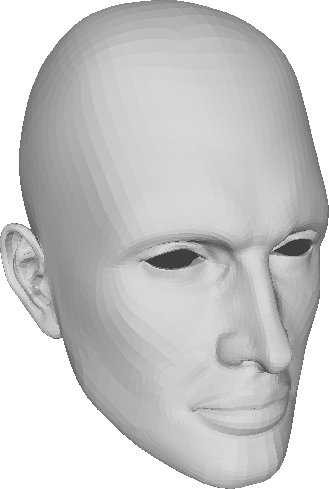
\includegraphics[width=0.65\linewidth]{images/maleHead}
  \end{center}
  \vspace{-10pt}
\caption{ The figure depicts a mesh of a male head. This head is used a test case for evaluating the smallest set grasp points needed for form fixture which also minimize the maximum contact wrench.}
  \vspace*{-10pt}
  \label{fig:maleHead}
\end{figure}

\begin{figure}[t!]
  \begin{center}
    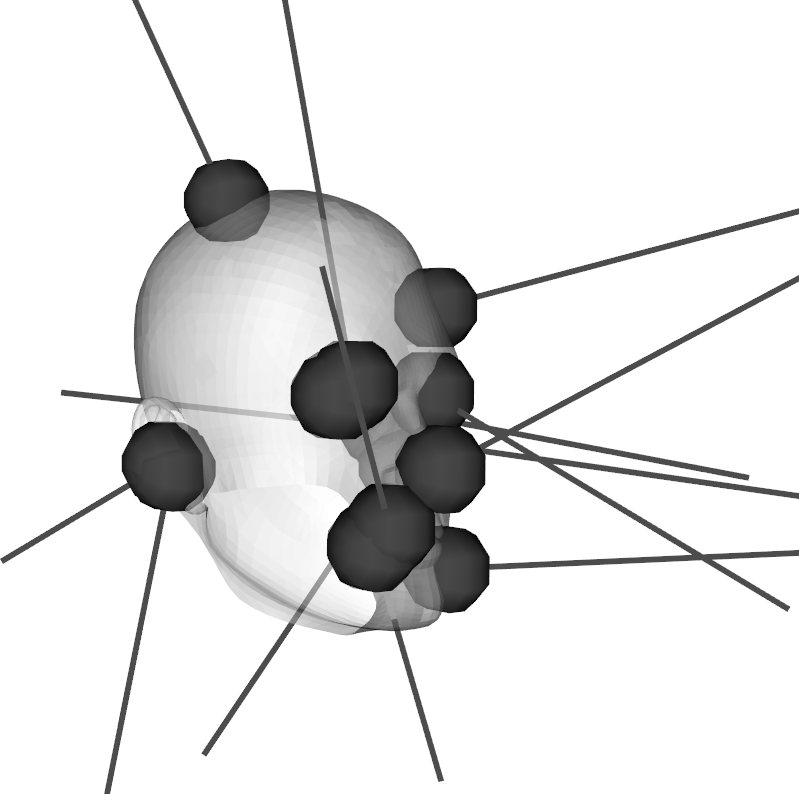
\includegraphics[width=0.75\linewidth]{images/maleHead-graspPoints-v1}
  \end{center}
  \vspace{-10pt}
\caption{ The figure depicts a set of grasp points generated for the aforementioned mesh of a male head. We note that the uniform sampling of candidate contact points results in pathological results. Hence we sample contact points as proposed in \ref{sec:Algorithm}}
  \vspace*{-15pt}
  \label{fig:maleHead-graspPoints}
\end{figure}
% Author: Animesh Garg
% Date: June 23, 2013

\section{DISCUSSION AND FUTURE WORK}

This is dummy text.


%%%%%%%%%%%%%%%%%%%%%%%%%%%%%%%%%%%%%%%%%%%%%%%%%%
%\section{CONCLUSION}
%Conclusion goes here.abbrvnat.bst

%%%%%%%%%%%%%%%%%%%%%%%%%%%%%%%%%%%%%%%%%%%%%%%%%%
%Keep this here for better formatting. 
\addtolength{\textheight}{-12cm}  
 % This command serves to balance the column lengths
% on the last page of the document manually. It shortens
% the textheight of the last page by a suitable amount.
% This command does not take effect until the next page
% so it should come on the page before the last. Make
% sure that you do not shorten the textheight too much.

%%%%%%%%%%%%%%%%%%%%%%%%%%%%%%%%%%%%%%%%%%%%%%%%%%
%% Author: Animesh Garg
% Date: June 23, 2013

\section*{APPENDIX}

Appendixes should appear before the acknowledgment.
%
%\section*{ACKNOWLEDGMENT}
%This is to thank people for their valuable support. 

%%%%%%%%%%%%%%%%%%%%%%%%%%%%%%%%%%%%%%%%%%%%%%%%%%
%References
%\bibliographystyle{IEEEtranS}
\bibliographystyle{ieeetr} %for use with natbib
\bibliography{graspSoft}

\end{document}